\section{Introduction to Signals and Systems}

\subsection{Introduction}

\begin{frame}{Introduction to the Course}
    \begin{itemize}[<+->]
        \item Signals and systems find many application in communications, automatic control, and form the basis for signal processing, machine vision, and pattern recognition.
        \item Electrical signals (voltages and currents in circuits, electromagnetic communication signals), acoustic signals, image and video signals, and biological signals are all example of signals that we encounter.
        \item They are functions of independent variables and carry information.
    \end{itemize}
\end{frame}

\begin{frame}{Introduction to Course Contd.}
    \begin{itemize}[<+->]
        \item We define a system as a mathematical relationship between an input signal and an output signal.
        \item We can use systems to analyze and modify signals.
        \item Signals and systems have brought about revolutionary changes.
        \item In this course we will study the fundamentals of signals and systems.
        \item Types of signals in continuous time and discrete time, linear time-invariant (LTI) systems, Fourier analysis, sampling, Laplace transform, $z$-transform, and stability of systems are the core components of the course.
    \end{itemize}
\end{frame}




\begin{frame}{Learning Outcomes}
    After completing this course you will be able to do the following:
    \begin{itemize}[<+->]
        \item Differentiate between continuous-time, discrete-time, and digital signals, and techniques applicable to the analysis of each type.
        \item Apply appropriate theoretical principles to characterize the behavior of linear time-invariant (LTI) Systems.
        \item Use Fourier techniques to understand frequency-domain characteristics of signals.
        \item Use appropriate theoretical principles for sampling and reconstruction of analog signals.
        \item Use the Laplace transform and the $z$-transform to treat a class of signals and systems broader than what Fourier techniques can handle.
    \end{itemize}
\end{frame}


\begin{frame}{Categories of Signals}
    \begin{itemize}[<+->]
        \item In this course we study signals and systems that process these signals.
        \item Categories of signals:
            \begin{itemize}
                \item Continuous-time signals: independent variable is continuous, $x(t)$
                \item Discrete-time signals:independent variable is an integer,  $x[n]$
            \end{itemize}
        \item There are some very strong similarities and also some very important differences between discrete-time signals and systems and continuous-time signals and systems.
    \end{itemize}
\end{frame}


\begin{frame}{Continuous-Time Signals $x(t)$}
    \begin{itemize}
        \item The independent variable is continuous.
        \item E.g., sound pressure at a microphone as a function of time (one-dimensional signal).
        \item E.g., image brightness as a function of two spatial variables (two-dimensional signal).
        \item Con convenience, we refer to the independent variable as time.
    \end{itemize}
\end{frame}

\begin{frame}[plain]
    \begin{columns}
        \begin{column}{0.6\textwidth}
            \begin{tikzpicture}
                \begin{axis}[
                    axis x line=middle,
                    axis y line=left,
                    no markers,
                    smooth,
                    y axis line style = {-stealth},
                    x axis line style = {-stealth},
                    x label style = {at={(ticklabel* cs:1.05)}, anchor=west, },
                    y label style = {at={(ticklabel* cs:1.1)}, anchor=north, rotate=-90,},
                    xlabel= {$t$},
                    ylabel={$x(t)$},
                    xticklabels={,,}]
                    \addplot table  [x=f, y=x, col sep=comma] {../Code/audioclip.csv};
                \end{axis}
            \end{tikzpicture}
        \end{column}
        \begin{column}{0.4\textwidth}
            A function of a continuous variable\\
            A speech signal: a continuous-time, one-dimensional signal\\
        \end{column}
    \end{columns}
\end{frame}


\begin{frame}[plain]


    \begin{columns}
        \begin{column}{0.6\textwidth}
            \begin{tikzpicture}
                \begin{axis}[
                    axis x line*=top,
                    axis y line*=left,
                    %x dir=reverse,
                    y dir=reverse,
                    enlargelimits=false,
                    y axis line style = {-stealth},
                    x axis line style = {-stealth},
                    xlabel= {$y$},
                    ylabel={$x$},
                    x label style = {at={(ticklabel cs:1)}, anchor=south west, },
                    %y label style = {at={(ticklabel cs:0)}, anchor=north, rotate=-90,},
                    ylabel=\empty,
                    xticklabels={,,},
                    yticklabels={,,},
                    xmin=0,xmax=295,
                    ymin=0,ymax=350,
                    axis on top,
                    axis equal image,
                    width=6cm,
                    clip=false,
                    ]
                    \addplot graphics [xmin=0,xmax=268,ymin=0,ymax=326] {figures/joseph_fourier.jpg};
                    \node at (axis cs: 134, 360 ) {$f(x,y)$};
                    \node at (axis cs: 0, 370 ) {$x$};
                \end{axis}
            \end{tikzpicture}
        \end{column}
        \begin{column}{0.4\textwidth}
            An image on a film: a continuous-time, two-dimensional signal\\
        \end{column}
    \end{columns}

\end{frame}

%\begin{frame}[plain]
%    \begin{tikzpicture}
%    \begin{axis}[
%    	title={Mesh on top of patches (i): obscured}]
%
%    \addplot3[patch,patch type=biquadratic,shader=interp,
%    	patch refines=3]
%    coordinates {
%    	(0,0,1) (6,1,1.6) (5,5,1.3) (-1,5,0)
%    	(3,1,0) (6,3,0.4) (2,6,1.1) (0,3,0.9)
%    	(3,3.75,0.5)
%    };
%    \addplot3[patch,patch type=biquadratic,mesh,black,
%    	patch refines=3]
%    coordinates {
%    	(0,0,1) (6,1,1.6) (5,5,1.3) (-1,5,0)
%    	(3,1,0) (6,3,0.4) (2,6,1.1) (0,3,0.9)
%    	(3,3.75,0.5)
%    };
%    \end{axis}
%    \end{tikzpicture}
%\end{frame}



% Topics to cover
% 1. Periodic vs. aperiodic
% 2. CT vs. DT
% 3. Energy vs. power signals

\begin{frame}[plain]{Discrete-Time Signals $x[n]$}
    \begin{itemize}
        \item Function of an integer variable.
        \item Takes on values at integer values of the argument of $x[n]$.
    \end{itemize}
    \begin{figure}
      \centering
      \begin{filecontents}{data.dat}
 n   xn 
-4   -1.0
-3   0.5 
-2  1.5  
-1   1.0  
 0    1.5  
 1    2.0  
 2    -2.0  
 3    1.0  
 4    0.0 
\end{filecontents}



\begin{tikzpicture}
\begin{axis}
[
    scale=1,
    axis x line=middle,
    axis y line=middle,
    every axis x label={at={(current axis.right of origin)},anchor=north west},
    every axis y label={at={(current axis.above origin)},anchor= north west},
    every axis plot post/.style={mark options={fill=black}},   
    xmin=-5.5,
    xmax=5.5, 
    xtick ={-4,-3,-2, -1, 0, 1, 2, 3, 4},
    xlabel={$n$},
    ylabel={$x[n]$},
    ytick={-2,-1, 0, 1, 2},   
    ymin=-2.5,
    ymax=2.5,
         every axis x label/.style={
    at={(ticklabel* cs:1.05)},
    anchor=west,
},
every axis y label/.style={
    at={(ticklabel* cs:1.05)},
    anchor=south,},
]
\addplot+[ycomb,black, thick] table [x={n}, y={xn}] {data.dat};
\end{axis}
\end{tikzpicture}
      \caption{DT Signal}\label{fi:dt_signal}
    \end{figure}
    \begin{itemize}
        \item E.g., weekly stock market index: a DT one-dimensional signal.
        \item E.g., image brightness,  $x[n,m]$,  as a function of the two spatial variables is a two-dimensional DT signal.
    \end{itemize}
\end{frame}

\begin{frame}{Digital Signals}
    \begin{itemize}
      \item What is a digital signal?
        \begin{itemize}
            \item A quantized discrete-time signal. I.e., $x[n,m]$ can take only a value from a finite set of values.
        \end{itemize}

      \item What is a digital image?
        \begin{itemize}
            \item A two-dimensional, quantized, discrete-time signal.
            \item A $600 \times 800$ image: $n \in [0, 599]$, $m \in [0, 799]$, $x[n,m] \in [0,255]$. 8-bit image.
        \end{itemize}
    \end{itemize}
\end{frame}

\begin{frame}{Systems}
    \begin{itemize}[<+->]
        \item A system processes signals.
        \item Examples of systems:
            \begin{itemize}
                \item Dynamics of an aircraft.
                \item An algorithm for analyzing financial and economic factors to predict bond prices.
                \item An algorithm for post-flight analysis of a space launch.
                \item An edge detection algorithm for medical images.
            \end{itemize}
    \end{itemize}
\end{frame}

\begin{frame}[plain]{CT and DT Systems}
\begin{figure}
    \centering
    %\begin{subfigure}[t]{0.5\textwidth}
        %\centering
        \begin{tikzpicture}
	\node (x) at (0,0) [anchor=east] {$x[n]$};
	\node (s) [draw, right=of x, minimum height=1cm, minimum width = 2cm] {System};
	\node (y) [right=of s] {$y[n]$};	
	\draw [-latex] (x) -- (s);
	\draw [-latex] (s) -- (y);
\end{tikzpicture}
        %\caption{CT system}
    %\end{subfigure}%
    %~
    %\begin{subfigure}[t]{0.5\textwidth}
        %\centering
        \begin{tikzpicture}
	\node (x) at (0,0) [anchor=east] {$x[n]$};
	\node (s) [draw, right=of x, minimum height=1cm, minimum width = 2cm] {System};
	\node (y) [right=of s] {$y[n]$};	
	\draw [-latex] (x) -- (s);
	\draw [-latex] (s) -- (y);
\end{tikzpicture}
        %\caption{DT system}
    %\end{subfigure}
    \caption{CT and DT Systems}\label{fi:ct_dt_systems}
\end{figure}
\end{frame}

\begin{frame}[plain]{Types of Systems}
    \begin{figure}
        \centering
        \begin{tikzpicture}[
  %man/.style={rectangle,draw,fill=blue!20},
  block/.style={rectangle,draw,fill=red!20,rounded corners=.8ex},
  grandchild/.style={grow=down,xshift=1em,anchor=west,
    edge from parent path={(\tikzparentnode.south) |- (\tikzchildnode.west)}},
  first/.style={level distance=6ex},
  second/.style={level distance=12ex},
  third/.style={level distance=18ex},
  level 1/.style={sibling distance=10em}]
    % Parents
    \node[block] {Systems}
      child[level distance=2ex]
    [edge from parent fork down]
    % Children and grandchildren
    child{node[block] {Linear}
      child[grandchild,first] {node[block]{Time-invariant}}
      child[grandchild,second] {node[block]{Time-variant}}}
    child{node[block] {Non-Linear}
      child[grandchild,first] {node[block]{Time-invariant}}
      child[grandchild,second] {node[block]{Time-variant}}};
\end{tikzpicture} 
        \caption{CT and DT Systems}\label{fi:system_types}
    \end{figure}
    This course is focused on the class of linear, time-invariant (LTI) systems.
\end{frame}


\begin{frame}{Examples of Systems}
    \begin{itemize}
      \item Dynamics of an aircraft.
      \item An algorithm for analyzing financial and economic factors to predict bond prices.
      \item An algorithm for post-flight analysis of a space launch.
      \item An edge detection algorithm for medical images.
    \end{itemize}
\end{frame}

\begin{frame}{Systems Interconnections}
    \begin{itemize}
      \item To build more complex systems by interconnecting simpler subsystems.
      \item To modify the response of a system.
      \item E.g.: amplifier design, stabilizing unstable systems.
    \end{itemize}
\end{frame}

\begin{frame}[plain]{Signal-Flow (Block) Diagrams}
    \begin{figure}
        \centering
        \tikzset{%
  block/.style    = {draw, rectangle, minimum height = 2em, minimum width = 4em, fill=red!20},
  sum/.style      = {draw, circle, node distance = 2cm}, % Adder
  io/.style    = {coordinate}, %input-output
    junction/.style    = {coordinate}
}
% Defining string as labels of certain blocks.
\newcommand{\suma}{\Large$+$}
\newcommand{\inte}{$\displaystyle \int$}
\newcommand{\derv}{\huge$\frac{d}{dt}$}

\begin{tikzpicture}[auto, node distance =2cm, >=triangle 45, scale=0.8]

	\begin{scope}
		\node (input) at (0,0) [io] {};
		\node (b1) [right of=input, block] {};
		\node (b2) [right of=b1, block] {};
		\node (output) [right of=b2, io] {};
		
		\draw[->](input) --  (b1);
		\draw[->](b1) --  (b2);
		\draw[->](b1) --  (b2); 	
		\draw[->](b2) --  (output);
		
		\node at (4, -1.1) {Series (Cascade)};		
	\end{scope}	
	
	\begin{scope}[yshift=-3.5cm]
		\node (input) at (0,0) [io] {};
		\node (j1) [right of=input, xshift=-1cm, junction] {};	
		\node (b1) [above of=j1, xshift=2cm, yshift=-1.25cm, block] {};
		\node (b2) [below of=j1, xshift=2cm, yshift=1.25cm, block] {};		
		\node (s1) [right of=b1, xshift=0cm, yshift=-0.75cm, sum] {$+$};				
		\node (output) [right of=s1, xshift=-1cm, io] {};
		
		
		\draw[] (input) --  (j1);		
		\draw[->] (j1) |-  (b1);	
		\draw[->] (j1) |-  (b2);	
		\draw[->] (b1) -|  (s1);	
		\draw[->] (b2) -|  (s1);
		\draw[->] (s1) --  (output);		
		\node at (4, -1.75) {Parallel};			
	\end{scope}
	
	
	\begin{scope}[yshift=-6.2cm]
		\node (input) at (0,0) [io] {};
		\node (s2) [right of=input, sum] {$+$};	
		\node (b3) [right of=s2, xshift=0cm, block] {};
		\node (j2) [right of=b3, xshift=-0.5cm,  junction] {};		
		\node (output) [right of=j2, xshift=-1cm, io] {};	
		\node (b4) [below of=b3, yshift=1cm, block] {};		

		
		
		\draw[->] (input) --  (s2);		
		\draw[->] (s2) --  (b3);	
		\draw[] (b3) --  (j2);
		
		\draw[->] (j2) --  (output);	
		\draw[->] (j2) |- (b4);		
		\draw[->] (b4) -| (s2);
		\node at (4, -2) {Feedback};			
	\end{scope}	
\end{tikzpicture} 
        \caption{System interconnections.}\label{fi:sys_interconnections}
    \end{figure}
\end{frame}


\begin{frame}[plain]{Domains}
    \begin{figure}
        \centering
        %\pgfplotsset{compat=1.12}
\pgfplotsset{every tick label/.append style={font=\scriptsize}}
\begin{filecontents}{data.dat}
 n   xn
-2  1.5
-1   1
 1    1
 2    1.5
\end{filecontents}
  \begin{tikzpicture}
  \def\omwga0{2*pi}
  \def\phase{0}
    \begin{axis}[
     clip=false,
     xmin=-3*pi,xmax=3*pi,
     xlabel= $t$,
     ylabel=$ x(t)$,
     ymin=-2.25,ymax=2.75,
     axis lines=middle,
     %axis x line=middle,
     %axis y line=left,
%     axis x line=middle,
     %xtick={-3.14, -1.57, 0,1.57,3.14,4.71,6.28, 7.85},
     %xticklabels={$-\pi$, $-\frac{\pi}{2}$, $0$, $\frac{\pi}{2}$,$\pi\,$,$\,\,\,\frac{3}{2}\pi$,$\,\,\,2\pi$, $\frac{5\pi}{2}$},
     ytick={-2.5, -2, -1.5, -1, -0.5, 0, 0.5, 1, 1.5, 2, 2.5},
     yticklabels={-2.5, -2, -1.5, -1, -0.5, 0, 0.5, 1, 1.5, 2, 2.5},
     %xticklabel style={anchor=north west}
     xticklabels=none,
     %xticklabel style={anchor=north west}
     %yticklabels=none,     
     every axis x label/.style={
    at={(ticklabel* cs:1.05)},
    anchor=west,
},
every axis y label/.style={
    at={(ticklabel* cs:1.05)},
    anchor=south,
},
     ]
      \addplot[domain=-2*pi:2*pi,samples=200,red]{cos(deg(x) + \phase) + 1.5*cos(2*deg(x)}
                                node[pos=1,font=\footnotesize, black]{\scriptsize $x(t) = \cos(t) + 1.5\cos(2t)$};
                                
                                
%        \draw[|-|] (axis cs: pi/4,1.1) -- (axis cs: 2*pi +pi/4,1.1) node[midway, above] {\scriptsize $T=\frac{2\pi}{\omega_0}$};
%        \node at (axis cs:0, .707) [anchor=east] {\scriptsize $A\cos\phi$  };
       
%        \node at (axis cs:pi, -1.2) [anchor=west] {\scriptsize $A =$ amplitude };
%        \node at (axis cs:pi, -1.4) [anchor=west] {\scriptsize $\omega_0 =$ frequency (here $\omega_0 =1$) };
%        \node at (axis cs:pi, -1.6) [anchor=west] {\scriptsize $\phi =$ phase (here $\phi =-\pi/4$) };
    \end{axis}
    
   \begin{scope}
       \begin{axis}
[%%%%%%%%%%%%%%%%%%%%%%%%%%%%%%%%%%%
    scale=1,
    axis x line=middle,
    axis y line=middle,
    every axis x label={at={(current axis.right of origin)},anchor=north west},
    every axis y label={at={(current axis.above origin)},anchor= north west},
    every axis plot post/.style={mark options={fill=black}},
    xmin=-3.5,
    xmax=3.5,
    xtick={-3, -2, -1, 1, 2, 3},
    xticklabels={$-3\omega_0$, $-2\omega_0$, $-\omega_0$, $\omega_0$, $2\omega_0$, $3\omega_0$},    
    xlabel={$\omega$},
    ylabel={$X(j\omega)/\pi$},
    ytick={0, 0.5,  1, 1.5},
    ymin=-1.25,
    ymax=1.75,
     every axis x label/.style={
    at={(ticklabel* cs:1.05)},
    anchor=west,
},
every axis y label/.style={
    at={(ticklabel* cs:1.05)},
    anchor=south,
},    
    xshift=8cm,
]%%%%%%%%%%%%%%%%%%%%%%%%%%%%%%%%%%%
\addplot+[ycomb,blue!70!black, mark=triangle*,mark options={rotate=180}] table [x={n}, y={xn}] {data.dat};
\end{axis}
\end{scope}

    
    
  \end{tikzpicture}
        \caption{Domains.}\label{fi:domains}
    \end{figure}
\end{frame}


\begin{frame}[plain]{Domains}
    \begin{figure}
        \centering
        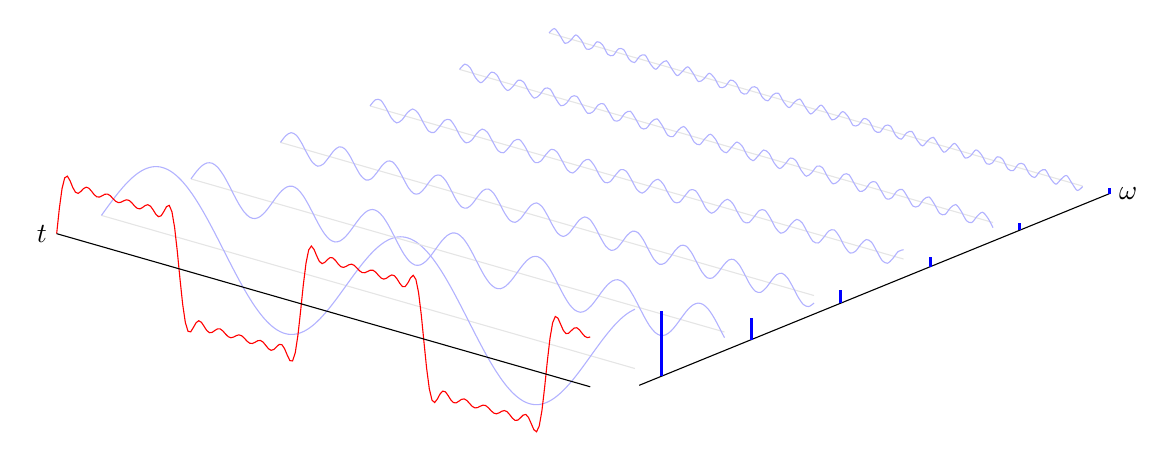
\begin{tikzpicture}
\begin{axis}[
    set layers=standard,
    domain=0:10,
    samples y=1,
    view={40}{20},
    hide axis,
    unit vector ratio*=1 2 1,
    xtick=\empty, ytick=\empty, ztick=\empty,
    clip=false,
    scale = 2,
]
\def\sumcurve{0}
\pgfplotsinvokeforeach{0.5,1.5,...,5.5}{
    \draw [on layer=background, gray!20] (axis cs:0,#1,0) -- (axis cs:10,#1,0);
    \addplot3 [on layer=main, blue!30, smooth, samples=101] (x,#1,{sin(#1*x*(157))/(#1*2)});

    \addplot3 [on layer=axis foreground, very thick, blue,ycomb, samples=2] (10.5,#1,{1/(#1*2)});
    \xdef\sumcurve{\sumcurve + sin(#1*x*(157))/(#1*2)}
}
\addplot3 [red, samples=200] (x,0,{\sumcurve});

\draw [on layer=axis foreground]  (axis cs:0,0,0) node [anchor=east] {$t$} -- (axis cs:10,0,0);
\draw (axis cs:10.5,0.25,0) -- (axis cs:10.5,5.5,0) node [anchor=west] {$\omega$};
\end{axis}
\end{tikzpicture} 
        \caption{Square wave: time and frequency domains.}\label{fi:square_wave_approx}
    \end{figure}
\end{frame}
